\section{Materiais e Métodos}
A partir do desenho de uma máquina síncrona apresentado na figura \ref{maq_sinc_id}, foi elaborada uma aplicação para o software de elementos finitos FEMM, utilizando a linguagem LUA para simular a seguinte condição: uma corrente Ic percorre os enrolamentos de campo da máquina síncrona. Deseja-se obter os gráficos de densidade de fluxo magnético, potencial elétrico e intensidade de campo a partir da simulação.
\begin{figure}[H]
\centering
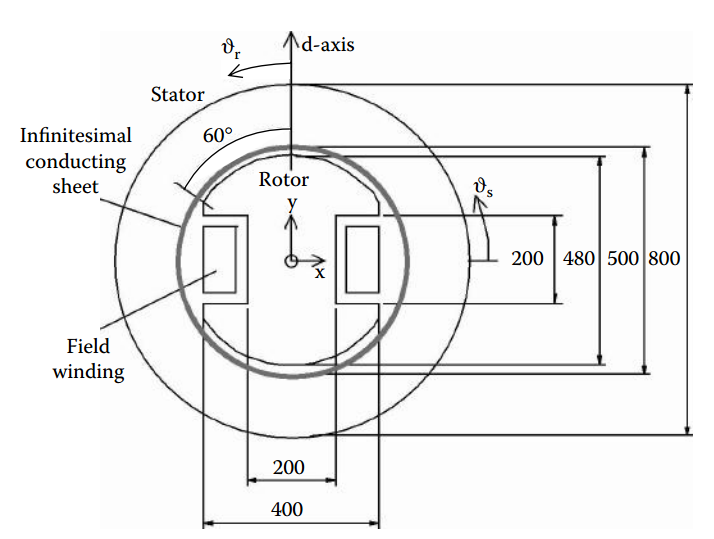
\includegraphics[scale=0.7]{img/assig4/ideal_synchronous_machine.png}
\caption[Representação de uma máquina síncrona]{Representação de uma máquina síncrona. Extraído de \cite{Bianc}.}
\label{maq_sinc_id}
\end{figure}
